\documentclass{beamer}
\usepackage{beamerthemesplit}
\usepackage{color}
\usepackage{amsfonts}
\usepackage{multimedia}
\usepackage{animate}
\usepackage{wrapfig}
\usepackage{multicol}
\setlength{\columnsep}{0cm}

\definecolor{cvggreen}{RGB}{4,71,79}
\mode<presentation>
{
%Darmstadt
\usetheme[]{Amsterdam}
}
\title{Marchiatura digitale di sequenze video stereoscopiche a disparit\`{a} coerente}
\author{Benedetta Barbetti\\ 
		Michaela Servi}
\institute{Universit\`{a} degli studi di Firenze}
\date{10 Dicembre 2015}


\begin{document}

\begin{frame}
\titlepage
\end{frame}

\begin{section}{Introduzione}
\subsection{Video Stereoscopici}

\begin{frame}[t]{\textsc{Contesto}}
Numerose applicazioni di elaborazione di immagini e video richiedono esplicite informazioni sulla \textbf{profondit\`{a}} della scena:
\begin{columns}
\begin{column}{4cm}
\begin{center}
%	\textbf{Caratteristiche}:
			\vspace*{0.5em}
			%\begin{small}
			\begin{itemize}
			\item \small{Medicina} 
			\item Robotica
			\item Tracking
			\item Industria manifetturiera
			\item Cinema
			\end{itemize}
			%\end{small}

\end{center}
\end{column}
\begin{column}{6cm}
\begin{figure}
\centering
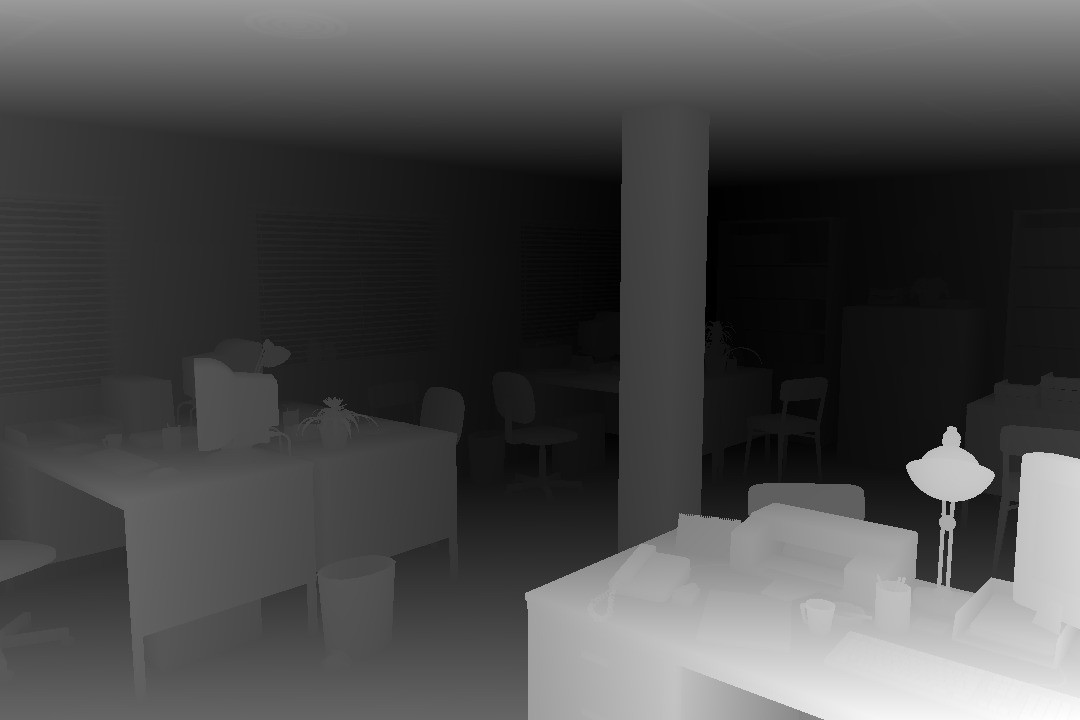
\includegraphics[width=1\linewidth]{./img/dm.jpg}
\end{figure}
\end{column}
\end{columns}
\end{frame}


\begin{frame}[t]{\textsc{Video Stereoscopici}}
	\setbeamertemplate{blocks}[rounded][shadow=false]
	\setbeamercolor{block title}{use=structure,fg=black,bg=lightgray} 
	\setbeamercolor{block body}{use=structure,fg=black,bg=lightgray} 	
\begin{block}
\centering

\end{block}
\movie[width=3cm,height=2cm,poster]{}{./img/alice.mp4}
\end{frame}


\begin{frame}[t]{\textsc{Dispositivi di ripresa e visualizzazione}}
	\vspace{1em}
\centering
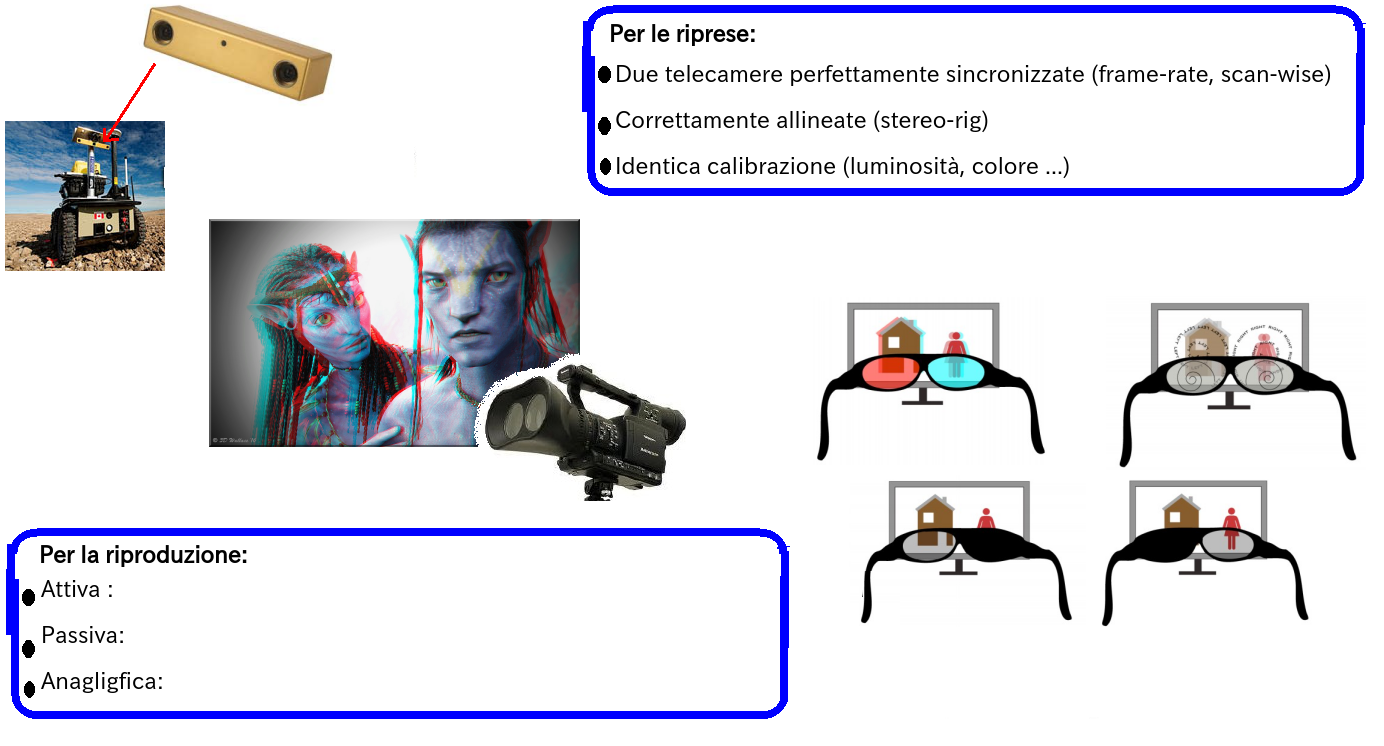
\includegraphics[width=1\linewidth]{./img/mah.png}
\end{frame}

\begin{frame}[t]{\textsc{Necessit\`{a} di una marchiatura}}

\end{frame}


\begin{frame}[t]{\textsc{Scopo di questa tesi}}

\end{frame}

\end{section}

\begin{section}{Stereoscopia}
\subsection{Principi della stereoscopia}
\begin{frame}[t]{\textsc{Stereoscopia}}

\end{frame}

\end{section}


\begin{section}{Watermarking}
\subsection {Principi del watermarking}
\begin{frame}[t]{\textsc{Watermarking}}

\end{frame}


\end{section}
\begin{section}{Stato dell'Arte}
\subsection{Watermarking di video stereoscopici}
\begin{frame}[t]{\textsc{Stato dell'arte}}

\end{frame}

\begin{frame}[t]{\textsc{Metodi a Disparit\`{a} Coerente}}
\end{frame}

\end{section}

\begin{section}{Metodo implementato}
\begin{frame}[t]{\textsc{Marchiatura digitale spaziale a disparit\`{a} coerente}}

\end{frame}
\end{section}




\end{document}
